% !TEX encoding = UTF-8
% !TEX TS-program = pdflatex
% !TEX root = ../thesis.tex

%************************************************
\chapter{The Standard Model of Particle Physics}\label{chap:two}
%************************************************

\section{Electroweak Symmetry breaking} \label{sec:2:EW_symmetry_breaking}
The standard model (\acs{SM}) of particle physics is a theory describing all known matter and their fundamental interactions except for gravity. It unifies the electromagnetic, weak, and strong forces under a single theoretical framework.
\begin{figure}
\centering
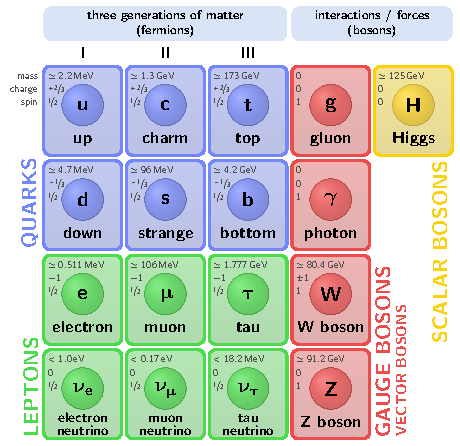
\includegraphics[width=0.7\textwidth]{Images/SM.pdf}
\caption{Elementary particles of the \acs{SM}. The was image generated with the help of Ref.~\cite{Neutelings_2024}.}
\label{fig:2:SM}
\end{figure}
The matter content of the \acs{SM} is classified into two primary groups: \textit{fermions} and \textit{bosons}. The fermions have spin $1/2$, they are further subcategorized into \textit{quarks} and \textit{leptons}. Quarks participate in strong interactions, while leptons interact only via the electromagnetic and weak forces. In contrast, bosons have integer spin. There exists a single particle with spin 0, the \textit{Higgs} boson, and four vector bosons, namely the gluon, the photon, and the $W$ and $Z$ boson. The vector bosons act as force carrier for the strong, the electromagnetic and the weak force respectively. Fermions are organized into three generations, with each generation containing two types of quarks (up-type and down-type) and two leptons (a charged lepton and its corresponding neutrino). These generations are shown in Fig.~\ref{fig:2:SM}, along with their masses, charges, and spins.

The interactions between \acs{SM} particles are described by a non-abelian gauge theory of the $\SU{3}_C \times \SU{2}_L \times \U{1}_Y$ group. Here $\SU{3}_C$ governs the strong interactions. It applies to all \textit{colored} particles, \ie~quarks and gluons. The quarks transform under the fundamental representation of the $\SU{3}_C$ group. $\SU{2}_L \times \U{1}_Y$ governs electroweak interactions. The $\SU{2}_L$ transformation acts non-trivially only on \textit{left-handed} fermions which form doublets
\begin{equation}
\begin{gathered}
L_{iL} \equiv \begin{pmatrix}
\nu_{iL} \\
l_{iL}
\end{pmatrix}, \quad Q_{iL} \equiv \begin{pmatrix}
u_{iL} \\
d_{iL}
\end{pmatrix}, \\
\nu_i = \left( \nu_e, \nu_\mu, \nu_\tau \right),\quad  l_i = \left( e, \mu, \tau \right),\quad u_i = \left(u, c, t \right),\quad d_i = \left(d, s, b \right).
\end{gathered}
\end{equation}
The phase transformation $\U{1}_Y$ acts on all particles except neutrinos according to their quantum number, the \textit{hypercharge} $Y$. The symmetry is spontaneously broken to $\SU{3}_C \times \U{1}_Q$, where the $\U{1}_Q$ group corresponds to gauge transformation of the electromagnetic interaction, hence the subscript $Q$ for the \textit{electric charge}. To ensure that the particles have the correct charges, the hypercharge must satisfy the \textit{Gell-Mann--Nishijima relation}:
\begin{equation}
\frac{Y}{2} = Q - I^3.
\end{equation}
With the particle charges displayed in Fig.~\ref{fig:2:SM} we then get
\begin{equation*}
\begin{tabular}{ccccccc}
  \hline
                & $L_{iL}$ & $Q_{iL}$ & $\nu_{iR}$ & $l_{iR}$ & $u_{iR}$ & $d_{iR}$ \\ \hline
  $\frac{Y}{2}$ & $-\frac{1}{2}$ & $\frac{1}{6}$ & $0$ & $-1$ & $\frac{2}{3}$ & $-\frac{1}{3}$ \\ \hline
\end{tabular}
\end{equation*}

The transformation properties of the gauge bosons is dictated by the covariance of the covariant derivative
\begin{equation}
\begin{gathered}
D_\mu \equiv \partial_\mu - i g A^a_\mu T_R^a - i g_2 W_\mu^a I^a + i g_Y \frac{Y}{2} B_\mu \\
T_R^a = \begin{cases} T^a \quad &\text{for quarks}, \\
  0 \quad &\text{for leptons},
\end{cases}
\qquad I^a = \begin{cases} \frac{\tau}{2} \quad &\text{for left-handed fermions}, \\
  0 \quad &\text{for right-handed fermions},
\end{cases}
\end{gathered}
\label{eq:2:covariant_derivative}
\end{equation}
where $T^a$ and $\tau^a$ are the \textit{Gell-Mann} and \textit{Pauli} matrices.

Before spontaneous symmetry breaking, the Lagrangian which governs the evolution of all matter fields must be invariant under the $\SU{3}_C \times \SU{2}_L \times \U{1}_Y$ gauge group. Up to a \Charge\Parity\ violating term\footnote{The absence of the \Charge\Parity\ violating term $\theta \frac{g^2}{64 \pi^2}\epsilon^{\mu \nu \alpha \beta} F^{a}_{\mu \nu} F^{a}_{\alpha \beta}$ is an unsolved problem of particle physics, known as the strong CP problem.} the SM Lagrangian is the most general mass-dimension four Lagrangian for the described particle content
\begin{equation}
\mathcal{L}_\mathrm{SM} = \mathcal{L}_G + \mathcal{L}_F + \mathcal{L}_Y + \mathcal{L}_H.
\end{equation}
The gauge-field Lagrangian $\mathcal{L}_G$ describes the free propagation and in the case of the non-abelian groups $\SU{3}_C$ and $\SU{2}_L$ also the self-interaction of the gauge bosons. It is given by
\begin{equation}
\begin{gathered}
\mathcal{L}_G = - \frac{1}{4} G^{a}_{\mu \nu} G^{a\, \mu\nu} - \frac{1}{4} W^a_{\mu \nu} W^{a\, \mu\nu} - \frac{1}{4} B_{\mu\nu} B^{\mu \nu}, \\
G^a_{\mu\nu} \equiv \partial_\mu A^a_\nu - \partial_\nu A^a_\mu + g f^{abc} A^b_\mu A^c_\nu, \\
W^a_{\mu\nu} \equiv \partial_\mu W^a_\nu - \partial_\nu W^a_\mu + g_2 \epsilon^{abc} W^b_\mu W^c_\nu, \\
B_{\mu\nu} \equiv \partial_\mu B_\nu - \partial_\nu B_\mu.
\end{gathered}
\end{equation}
The propagation of the fermions and their interaction with the gauge bosons is described by
\begin{equation}
\mathcal{L}_F = \bar{L}_{iL} i \slashed{D} L_{iL} + \bar{\nu}_{iR} i \slashed{D} \nu_{iR} + \bar{l}_{iR} i \slashed{D} l_{iR} + \bar{Q}_{iL} i \slashed{D} Q_{iL} + \bar{u}_{iR} i \slashed{D} u_{iR} + \bar{d}_{iR} i \slashed{D} d_{iR}.
\end{equation}

The Higgs field is a doublet of the $\SU{2}_L$ group. We want the field to have a non-vanishing vacuum expectation value (\acs{VEV}) to dynamically generate the fermion and boson masses. Of course, the vacuum cannot carry an electric charge, which means that the Higgs field must be electrically neutral along the direction of \textit{spontaneous symmetry breaking} (\acs{SSB}). We choose this to be the second component of the doublet. With the Gell-Mann--Nishijima relation we can then deduce that hypercharge of the doublet must be $Y = +1$. The Higgs doublet field thus takes the form
\begin{equation}
\Phi = \begin{pmatrix}
  \phi^+ \\
  \phi^0
\end{pmatrix},
\end{equation}
where the superscript indicates the electic charge.

In order to generate a non-vanishing \acs{VEV}, the Higgs field must be in a potential with a global minimum away from zero. Hence, the only gauge invariant mass-dimension four Lagrangian we can construct is
\begin{equation}
\begin{gathered}
\mathcal{L}_H = \left( D_\mu \Phi \right)^\dagger \left( D^\mu \Phi \right) - V(\Phi) \\
V(\Phi) = \lambda (\Phi^\dagger \Phi )^2 - \mu^2 \Phi^\dagger \Phi, \quad \mu^2, \lambda > 0.
\end{gathered}
\end{equation}
The minimum of the Higgs potential $V$ is at
\begin{equation}
\Phi_0^\dagger \Phi_0 = \frac{\mu^2}{2 \lambda} \equiv \frac{v^2}{2} \neq 0.
\end{equation}
After (\acs{SSB}) we can expand the Higgs field around its minimum
\begin{equation}
\Phi = \begin{pmatrix}
  \phi^+ \\
  \frac{1}{\sqrt{2}} ( v + H + i \xi ).
\end{pmatrix}
\end{equation}
The real scalar field $H$ is the famous Higgs boson, whereas the fields $\phi^\pm$ and $\xi$ are unphysical since they can always be eliminated through a gauge transformation (\textit{would-be Goldstone bosons}). After inserting the expansion in the Higgs Lagrangian, the mass of the Higgs can be read off from its square term
\begin{equation}
m_H = \sqrt{2} \mu.
\end{equation}

\acs{SSB} enables the generation of vector boson masses without breaking the gauge symmetry explicitly. If we insert the expanded Higgs field in the Higgs Lagrangian, we get quadratic terms of the gauge boson fields
\begin{equation}
\begin{split}
\mathcal{L}_H &\supsetneq \frac{v^2}{2} \bigg \lbrace g_2^2 \begin{pmatrix} 0 & 1 \end{pmatrix} I^a I^b \begin{pmatrix} 0 \\ 1 \end{pmatrix} W^a_\mu W^{b\, \mu} - g_2 g_Y \begin{pmatrix} 0 & 1 \end{pmatrix} I^a \begin{pmatrix} 0 \\ 1 \end{pmatrix} W_\mu^a B^\mu + \frac{g_Y^2}{4} B_\mu B^\mu \bigg \rbrace \\
&= \frac{v^2}{2} \bigg \lbrace \frac{g_2^2}{4} \left[ (W^1)^2 + (W^2)^2 \right] + \frac{1}{4} \begin{pmatrix} B^\mu & W^{3\, \mu} \end{pmatrix} \begin{pmatrix}  g_Y^2 & g_Y g_2 \\ g_Y g_2 & g_2^2 \end{pmatrix} \begin{pmatrix} B_\mu \\ W^3_\mu \end{pmatrix} \bigg \rbrace.
\end{split}
\end{equation}
By diagonalizing the mass matrix we obtain the physical states
\begin{equation}
\begin{gathered}
\begin{pmatrix}
A^\gamma_\mu \\
Z_\mu
\end{pmatrix} = \begin{pmatrix}
\cos \theta_W & - \sin \theta_W \\
\sin \theta_W & \cos \theta_W
\end{pmatrix} \begin{pmatrix}
B_\mu \\
W_\mu^3
\end{pmatrix}
\end{gathered}, \quad \cos \theta_W = \frac{g_2}{\sqrt{g_Y^2 + g_2^2}}, \sin \theta_W = \frac{g_Y}{\sqrt{g_Y^2 + g_2^2}}.
\end{equation}
In this new basis, we have one massless boson $A^\gamma_\mu$, which we identify as the photon and a charge neutral boson of mass
\begin{equation}
m_Z = \frac{v}{2} \sqrt{g_Y^2 + g_2^2}.
\end{equation}
The vector bosons $W^1$ and $W^2$ are not eigenstates of the charge operator. We therefore define the new states
\begin{equation}
W^\pm_\mu = \frac{1}{\sqrt{2}} \left( W^1_\mu \mp i W^2_\mu \right), \qquad Q W_\mu^\pm = \pm W_\mu^\pm,
\end{equation}
which are eigenstates of $Q$ and have mass
\begin{equation}
m_W = \frac{v}{2} g_2.
\end{equation}

Last but not least, we discuss the Yukawa sector of the \acs{SM} Lagrangian. Before \acs{SSB}, fermions cannot generate masses because a mass term would mix the left- and right-handed components of the fields, thereby breaking the chiral gauge symmetry. Here, once again, the Higgs field comes to the rescue: by coupling the fermions with the Higgs field through a Yukawa interaction\footnote{In the original formulation of the \acs{SM}, there are no neutrino Yukawa interactions, since they were believed to be massless. Neutrino oscillation experiments have shown however, that neutrinos do in fact have finite masses.}
\begin{equation}
\mathcal{L}_Y = - \left( y_{ij}^\nu \bar{L}_{iL} \Phi^c \nu_{jR} + y_{ij}^l \bar{L}_{iL} \Phi l_{jR} + y_{ij}^d \bar{Q}_{iL} \Phi d_{jR} + y_{ij}^u \bar{Q}_{iL} \Phi^c u_{jR} \right) + \hc,
\end{equation}
where $\Phi^c$ is the charge-conjugated field to $\Phi$, we do not explicitly break the symmetry. However, after \acs{SSB} this Lagrangian will generate exactly the required mixing between left- and right-handed fields to generate the fermion masses. The Yukawa-interaction matrices $y_{ij}^{\nu,l, d, u}$ can be shifted from the Yukawa sector to the fermion sector through a field redefinition. Indeed, if we apply the \textit{singular value decomposition} of the Yukawa matrix
\begin{equation}
y = U_L^\dagger y_{\mathrm{diag}} U_R, \quad \text{with} \quad (y_{\mathrm{diag}})_{ij} = \sqrt{2} Y_i \delta_{ij} \quad \text{and} \quad U_{L,R} \in \U{3},
\end{equation}
and redefine our fermion fields to be
\begin{equation}
f_{iR} \longrightarrow U_{Rij} f_{jR}, \qquad f_{iL} \longrightarrow U_{Lij} f_{jL}, \qquad f = \nu, l, u, d
\end{equation}
the Yukawa Lagrangian becomes
\begin{equation}
\mathcal{L}_Y = - \sum_{i}\left( m_{\nu_i} \bar{\nu}_i \nu_i + m_{l_i} \bar{l}_i l_i + m_{u_i} \bar{u}_i u_i + m_{d_i} \bar{d}_i d_i \right)  \left(1 + \frac{H}{v} \right).
\label{eq:2:Yukawa_sector}
\end{equation}
Here we identified the Yukawa coupling as $Y_i = m_i/v$ in order to generate the required mass terms. Consequently, we observe that the Yukawa coupling of the Higgs to the fermions is proportional to the mass of that fermion.
The field redefinition is a change from a flavor eigenbasis, which is diagonal in the couplings to the gauge bosons, to a mass eigenbasis. In the mass eigenbasis the part of fermion Lagrangian which contains the interaction to the electroweak gauge bosons after SSB is
\begin{equation}
\begin{split}
\mathcal{L}_F \supsetneq &\sum_f (-Q_f) e \bar{f}_i \slashed{A}^\gamma f_i + \sum_f \frac{e}{\sin \theta_W \cos \theta_W} \bar{f}_i ( I_f^3 \gamma^\mu P_L - \sin^2 \theta_W Q_f \gamma^\mu) f_i Z_\mu \\
&+ \frac{e}{\sqrt{2} \sin \theta_W} \left( \bar{u}_i \gamma^\mu P_L (V_\mathrm{CKM})_{ij} d_j W_\mu^+ + \bar{d}_i \gamma^\mu P_L (V_{\mathrm{CKM}}^\dagger)_{ij} u_j W_\mu^- \right) \\
&+ \frac{e}{\sqrt{2} \sin \theta_W} \left( \bar{\nu}_i \gamma^\mu P_L (V_\mathrm{PMNS}^\dagger)_{ij} l_j W_{\mu}^+ + \bar{l}_i \gamma^\mu P_L (V_\mathrm{PMNS})_{ij} v_j W_\mu^- \right).
\end{split}
\end{equation}
Here we identified the electromagnetic coupling constant
\begin{equation}
e = \frac{g_2 g_Y}{\sqrt{g_2^2 + g_Y^2}},
\end{equation}
as the factor in front of the photon interaction term. The operators $P_{L,R}$ are just the projectors onto the left- and right-handed components
\begin{equation}
P_{L,R} = \frac{1 \mp \gamma^5}{2}.
\end{equation}
The \textit{CKM} and \textit{PMNS matrices}\footnote{Named after Cabibbo, Kobayashi and Maskawa, and Pontecorvo, Maki, Nakagawa and Sakata.} are the results of the field redefinitions
\begin{equation}
V_\mathrm{CKM} \equiv {U_L^{u}}^\dagger U_L^d, \qquad V_\mathrm{PMNS} \equiv {U_L^{l}}^\dagger U_L^\nu.
\end{equation}
Typically, one prefers to work in the mass eigenbasis of the quarks, while the neutrinos are kept in the flavor eigenbasis, in which case one encounters flavor changes (\textit{neutrino oscillations}) through propagation. This is why the PMNS matrix is defined in terms of the complex conjugate of the CKM matrix equivalent in the lepton sector.



\section{Cross Sections} \label{sec:2:cross_sections}
Cross sections offer the possibility to directly test the \acs{SM} and many of the great successes of the \acs{SM} are its \textit{cross section} predictions. The cross section is simply defined as the probability to create some final state from some initial state per unit of time per target particle normalized by the incoming particle flux. This definition allows for straightforward measurement through counting experiments. For instance, experiments like \texttt{CMS} and \texttt{ATLAS} collide particles and count how often a particular final state is produced within a given time interval.

From a theoretical perspective, cross sections can be calculated using
\begin{equation}
\dd \hat{\sigma}_{ij \rightarrow n} = \frac{1}{F} \dd \Phi_n |M_{ij\rightarrow n}|^2,
\label{eq:2:Xsec}
\end{equation}
where $F$ denotes the \textit{flux factor}\footnote{In the following we assume that the initial state particles are massless.}
\begin{equation}
F \equiv 4 p_1 \cdot p_2,
\end{equation}
$\dd \Phi_n$ is the \textit{Lorentz invariant phase space measure}
\begin{equation}
\dd \Phi_n = \left[\prod_{i = 1}^n \frac{\dd^4 q_i}{(2 \pi)^4 } (2 \pi) \delta(q_i^2 - m_i^2) \Theta(q_i^0) \right] (2 \pi)^4 \delta^{(4)} \! \left(p_1 + p_2 - \sum_{i = 1}^n q_i \right),
\end{equation}
and $M_{fi}$ is the \textit{scattering amplitude} describing the short distance interactions.

The computation of cross sections involves three basic steps:
\begin{enumerate}
  \item Calculation of the hard scattering amplitude,
  \item Phase-space integration,
  \item And the convolution with \textit{parton distribution functions} (\acs{PDF}s).
\end{enumerate}
We will discuss each step in detail below.

\subsection{The Hard Scattering Amplitude}
The Hard Scattering Amplitude describes the transition probability from a specific initial state to a particular finial state. Since the scattering is \textbf{hard}, it implies that the energy transfer between particles during scattering is large compared to the QCD scale. Thus, we operate within the perturbative regime of QCD and can perform an expansion in terms of the coupling constant
\begin{equation}
M_{ij \rightarrow n} = \alphas^{n_\text{Born}} \left( M_{ij \rightarrow n}^{(0)} + \frac{\alphas}{\pi} M_{ij \rightarrow n}^{(1)} + \left(\frac{\alphas}{\pi}\right)^2 M_{ij \rightarrow n}^{(2)} + \BigO{\alphas^3} \right).
\end{equation}
Here, $n_\text{Born}$ denotes the power of the coupling constant at \textit{leading order} (\acs{LO}). The coefficients in this series can be computed graphically using \textit{Feynman rules}. These are the set of all allowed propagators and vertices together with the corresponding mathematical prescription. The Feynman rules for the complete \acs{SM} are listed in Appendix~\ref{app:1}. To calculate the coefficient $M_{ij \rightarrow n}^{(l)}$ for a specific process, one has to draw all possible connected and amputated Feynman diagrams with the initial state $(i,j)$ and final state $n$, that contain $2(n_\text{Born} + l)$ vertices\footnote{Quartic vertices are counted twice.}. Then one uses the Feynman rules to get the mathematical translation, keeping in mind that momentum must be conserved at every vertex and also taking into account possible symmetry factors.

Starting from $M^{(1)}_{ij \rightarrow n}$, but for some processes, called \textit{loop induced processes}, even from $M^{(0)}_{ij \rightarrow n}$, we will encounter loops in the diagrams. Inside a loop, the momentum of the edges cannot be uniquely determined through momentum conservation. Consequently, we must leave momentum unspecified and integrate over all possible values. Typically, it is the computation of these \textit{loop integrals} that makes the calculation of hard scattering amplitudes so challenging. A plethora of powerful techniques has been developed over the years to tackle this daunting task. Still, the computation of loop integrals remains a highly active field of research and two-loop amplitudes with 5 or more scales are only just becoming available. A detailed description of modern techniques is beyond the scope of this thesis. For a comprehensive overview see Ref.~\cite{Weinzierl:2022eaz}.

Loop integrals are notorious for exhibiting divergences. To tame these, we introduce \textit{regulators}, \ie\ we introduce a parameter, such that the integral becomes function of that parameter with a singularity at the physical value. The most commonly used regularization scheme is \textit{dimensional regularization} (\acs{DR}), here we make the loop-integral a function of the dimension by replacing
\begin{equation}
\int \frac{\dd^4 k}{(2 \pi)^4} \left( \cdots \right) \longrightarrow \muBar^{2 \epsilon} \int \frac{\dd^d k}{(2 \pi)^d} \left( \cdots \right), \quad d \equiv 4 - 2 \epsilon \in \mathbb{C}, \quad \gamma_E =  0.5772\ldots.
\end{equation}
The dimensionally regularized integral satisfies the usual integral properties like linearity, translation invariance and rescaling. The mass scale,
\begin{equation}
\muBar^2 = \frac{\mu^2}{4 \pi} e^{\gamma_E}
\end{equation}
was introduced to retain the mass dimension of the measure to 4, while absorbing some common factors of loop integrals. The physical limit then corresponds to $\epsilon \rightarrow 0$. A divergent integral in four dimensions will hence have $\epsilon$-poles in \acs{DR}. The poles are categorized as \textit{ultraviolet} poles if their origin are large loop momenta, \ie\ the four dimensional integral diverges for $k \rightarrow \infty$. Further we categorize poles as \textit{infrared} poles if the singularity arises from loop momenta which are either \text{soft} ($k \rightarrow 0$) or \textit{collinear} ($k \cdot p_i \rightarrow 0$) to one of the external massless legs. \acs{UV} and \acs{IR} singularities are mutually exclusive since they originate from different regions of the phase space. This means that the poles do not multiply together, and we may only get a single \acs{UV} pole per loop integration. The soft and collinear singularities are \textbf{not} exclusive, meaning that \acs{IR} singularities can develop one double pole per loop integration.

The \acs{IR} singularities cancel for inclusive observables as we shall discuss in detail in section~\ref{subsec:2:phase_space_integration}. \acs{UV} poles on the other hand, are removed through a method called \textit{renormalization}. Renormalization hinges on the idea, that the fields, constants and masses we observe in nature are not necessarily the same as the one in our Lagrangian. Instead, they are related through a \textit{renormalization constant}
\begin{equation}
\begin{split}
W_\mu^{B,a} &= \left(Z_3^W \right)^{1/2} W_\mu^{R,a} \\
B_\mu^{B} &= \left(Z_3^Z \right)^{1/2} B_\mu^{R} \\
A_\mu^{B,a} &= \left(Z_3^A \right)^{1/2} A_\mu^{R,a} \\
\Phi^{B} &= \left(Z^\Phi \right)^{1/2} \Phi^{R} \\
Q_{iL}^{B} &= \left(Z_{2i}^L \right)^{1/2} Q_{iL}^{R} \\
u_{iR}^{B,a} &= \left(Z_{2i}^{u,R} \right)^{1/2} u_{iR}^{B,a} \\
d_{iR}^{B,a} &= \left(Z_{2i}^{d,R} \right)^{1/2} d_{iR}^{B,a} \\
g^B &= Z_g g^R \\
g_Y^B &= Z_Y g_Y^R \\
g_2^B &= Z_2 g_2^R \\
\left(\mu^2 \right)^B &= Z_\mu \left( \mu^2 \right)^R \\
\lambda^B &= Z_\lambda \lambda^R \\
y_{ij}^{d,B} &= Z_{y,ij}^{d} y_{ij}^{d,R} \\
y_{ij}^{u,B} &= Z_{y,ij}^{u} y_{ij}^{u,R} \\
\label{eq:2:renormalization}
\end{split}
\end{equation}
In these equations $B$ refers to \textit{bare} quantities appearing within our Lagrangian while $R$ signifies renormalized quantities that are finite by definition. In the \acs{SM}, it can be shown~\cite{tHooft:1971qjg,tHooft:1972tcz} that we can choose renormalization constants, such that \textit{Green's functions}, \ie\ vacuum expectation values of time ordered products of local renormalized fields, are free of \acs{UV} divergences. Scattering amplitudes, generally do not depend on the unphysical fields, which is why the fields can be kept unrenormalized in this case. Since at \acs{LO} Green's functions do not require renormalization, all renormalization constants are equal to the identity at this order.

The definition of the renormalization constants is not unique. Indeed, the renormalization constants were designed to absorb singularities, but the finite part is a priori unconstrained. We call a prescription which uniquely determines the renormalization constants a \textit{renormalization scheme}. The most widely used renormalization scheme is the \MS\ scheme. Here, beyond the leading $1$ and a universal factor of $\muBar^{\epsilon \rho_i}$, the renormalization constants \textbf{only} consist of poles, \ie\ the renormalization constants have the structure
\begin{equation}
Z_i(\alpha) = \muBar^{\epsilon \rho_i} \left(1 + \frac{z_1}{\epsilon} \frac{\alpha}{4 \pi} + \left(\frac{z_{22}}{\epsilon^2} + \frac{z_{21}}{\epsilon} \right) \left( \frac{\alpha}{4 \pi} \right)^2 + \dots \right).
\end{equation}
$\rho_i$ is the mass dimension of the operator in units of $\epsilon$, so that the factor $\muBar^{\epsilon \rho_i}$ corrects for the mismatch in mass dimensions between the four-dimensional renormalized and the $d$-dimensional bare quantities. For example: the coupling constant $g^B$ has mass dimension $\epsilon$, hence the renormalized coupling $g^R$ has mass dimension zero and $\rho_i = 1$.

\MS-renormalized masses are generally different from the pole mass. The \textit{on-shell renormalization} (\acs{OS}) scheme, is an alternative to the \MS\ scheme specifically designed, such that the renormalized mass matches the pole mass. It is therefore the suitable choice for external particles that are asymptotically free. Bare quantities are independent of the chosen renormalization scheme. The invariance under the change of the renormalization scheme defines a group, the \textit{renormalization group} (\acs{RG}). In the \MS\ scheme, the change from one scale $\muBar$ to another defines a continuous subgroup of the \acs{RG}. This means we can formulate the invariance in terms of a differential equation
\begin{equation}
0 = \frac{\dd}{\dd \log \mu} a^B  = a^R \frac{\dd Z^{\MS}_a}{\dd \log \mu} + Z^{\MS}_a \frac{\dd a^R}{\dd \log \mu},
\label{eq:2:RGE}
\end{equation}
where $a$ could be a mass or a coupling. Eq.~\eqref{eq:2:RGE} is called the \textit{renormalization group equation} (\acs{RGE}) and it can be leveraged to determine the scale dependence, also called the \textit{running}, of the observable.

The final step in calculating the hard scattering amplitude involves the application of the \textit{Lehmann-Symanzik-Zimmermann} (LSZ) reduction formula. It relates the scattering amplitudes to Green's functions, and it is the reason why we only considered amputated Feynman diagrams. In practice, one just has to multiply each external field with the square root of the corresponding LSZ constant. These constants are defined as the proportionality factor between the propagator of the interacting and the free theory\footnote{The interacting field theory might have an additional continuous spectrum.}. As such, they are numerically identical to the \acs{OS} field renormalization constants.

\subsection{The Parton Distribution Functions}\label{subsec:PDFs}
In hadron collisions, the initial state is not made up of elementary particles, but are bound states thereof. This means that during an inelastic scattering event, the partons which take part in the short-range interaction only carry a fraction of the original hadron momentum
\begin{equation}
p_1 = x_1 P_1, \qquad p_2 = x_2 P_2.
\end{equation}
Here $p_1$ and $p_2$ denote the momenta of the partons and $P_1$ and $P_2$ are the momenta of the hadrons. Since the momentum of the parton can not be larger than that of the hadron, $x_{1,2}$ is restricted to be less than one. Furthermore, since the energy of the parton must be positive the momentum fraction must also be positive. Otherwise, the momentum fraction is a priori unconstrained, we therefore integrate over all allowed values of $x_1$ and $x_2$
\begin{equation}
\begin{split}
\dd \sigma_{H_1 H_2 \rightarrow n}(S) &=  \int_0^1 \dd x_1 \dd x_2 \, f_{H_1,i}(x_1) f_{H_2, j}(x_2) \dd \hat{\sigma}_{ij \rightarrow n}(x_1 P_1, x_2 P_2, \mu_R) \\
&= \int_0^1 \frac{\dd \tau}{\tau} \mathcal{L}_{ij}(\tau) \dd \hat{\sigma}_{ij \rightarrow n}\!\left(\tau S, \mu_R \right)
\end{split}
\label{eq:2:factorization}
\end{equation}
where $S =2 P_1 \cdot P_2$ is hadronic center of mass energy. $f_{H_{k}, i}(x_k)$ are the (unrenormalized) \textit{parton distribution functions} (\acs{PDF}s). They describe the probability of finding a parton $i$ with momentum fraction $x_k$ inside the hadron $H_k$. Lorentz invariance of the partonic cross section allowed us to conclude that it can only depend on the partonic center of mass energy $\hat{s}$
\begin{equation}
\dd \hat{\sigma}_{ij \rightarrow n} (x_1 P_1, x_2 P_2, \mu_R) = \dd \hat{\sigma}_{ij \rightarrow n}(x_1 x_2 S, \mu_R).
\end{equation}
We then defined the \textit{partonic luminosity}
\begin{equation}
\mathcal{L}_{ij}(\tau) \equiv  (\tilde{f}_{H_1,i} \otimes \tilde{f}_{H_2,j})(\tau) \equiv \int_0^1 \dd x_1 \dd x_2 \, \tilde{f}_{H_1,i}(x_1) \tilde{f}_{H_2, j}(x_2) \delta(\tau - x_1 x_2),
\end{equation}
where $\tilde{f}_{H, i}(x) \equiv x f_{H, i}(x)$, to arrive at the second line of Eq.~\eqref{eq:2:factorization}.

At this stage the partonic cross section can still exhibit singularities whenever a finial state parton becomes collinear to one of the initial state partons. At \acs{LO} for example, the divergence due to initial-state collinear emissions reads
\begin{equation}
\dd \hat{\sigma}_{a b \rightarrow c X}(s, \mu_R) \Big\vert_{\text{div.}} = - \frac{\alphas}{2 \pi} \frac{1}{\epsilon}  \int_0^1 \dd z\, \left(P_{db}^{(0)}(z) \dd \hat{\sigma}_{a d \rightarrow X}(z s, \mu_R) + P_{da}^{(0)}(z) \hat{\sigma}_{d b \rightarrow X}(zs, \mu_R) \right),
\label{eq:2:initialDiv}
\end{equation}
where $P_{ij}^{(0)}$ are the \acs{LO} \textit{Altarelli-Parisi splitting kernels}\footnote{The definition of $\beta_0$ can be found in Eq.~\eqref{eq:4:beta0_and_beta1}}:
\begin{equation}
\begin{split}
&P_{qq}^{(0)}(x) = C_F \left[ \frac{1 + x^2}{(1 - x)_+} + \frac{3}{2} \delta (1 - x) \right], \\[3mm]
&P_{qg}^{(0)}(x) = T_F \left[ x^2 + (1 - x)^2 \right], \\[3mm]
&P_{gq}^{(0)}(x) = C_F \left[ \frac{1 + (1 - x)^2}{x} \right], \\[2mm]
&P_{gg}^{(0)}(x) = 2C_A \left[ \frac{x}{(1 - x)_+} + \frac{1 - x}{x} + x (1 - x) \right] + \delta(1 - x) \frac{\beta_0}{2}.
\end{split}
\label{eq:2:Altarelli_Parisi_splitting_functions}
\end{equation}

We absorb these collinear singularities into the PDFs through a process called \textit{collinear renormalization}, by defining the renormalized \acs{PDF}s $f_{H, i}(x, \mu_F)$ via
\begin{equation}
f_{H, i}(x) \equiv (Z_{ij}(\cdot, \mu_F) \otimes f_{H, j}(\cdot, \mu_F))(x).
\end{equation}
Beyond the pole term, the renormalization constants are generally scheme dependent. From Eq.~\eqref{eq:2:initialDiv} we see that the \MS\ renormalization constant at NLO are given by
\begin{equation}
Z_{ij}(z, \mu_R, \mu_F) = \delta(1 - z) \delta_{ij} + \frac{\alphas}{2 \pi} \frac{1}{\epsilon} P_{ij}^{(0)}(z) + \BigO{\alphas^2}.
\end{equation}
Now the sum
\begin{equation}
\dd \sigma_{H_1 H_2 \rightarrow c X} + \dd \sigma_{H_1 H_2 \rightarrow X}
\end{equation}
is guaranteed to be free initial-state collinear divergences.

Since the initial state collinear divergences are of a completely different origin than the \acs{UV} divergences, we introduce a new scale $\mu_F$, called the factorization scale. This scale separates the long-distance (non-perturbative) physics, contained in the PDFs, from the short-distance (perturbative) physics, contained in the partonic cross sections.

\begin{figure}[h]
\begin{minipage}[t]{0.48\textwidth}
\centering
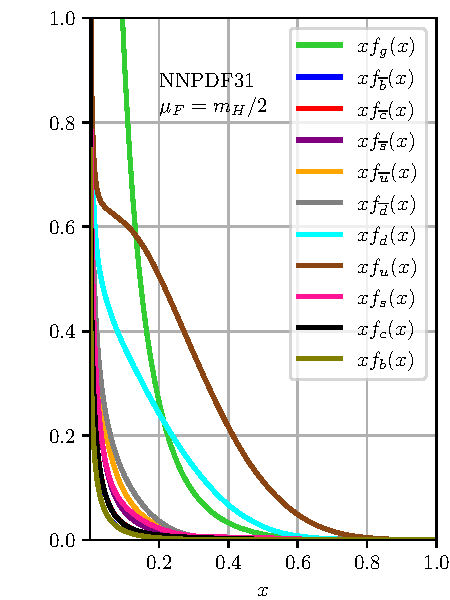
\includegraphics[width=\textwidth]{Images/PDF.pdf}
\captionof{figure}{The various \acs{PDF}s multiplied by $x$ as a function of $x$. The plot was created using the \texttt{LHAPDF6}~\cite{Buckley:2014ana} interface to the \texttt{NNPDF31\_nnlo\_as\_0118}~\cite{NNPDF:2017mvq} \acs{PDF} set at a scale of $\mu_F=m_H/2$.}
\label{fig:2:PDF}
\end{minipage}
\hspace{0.02\textwidth}
\begin{minipage}[t]{0.48\textwidth}
\centering
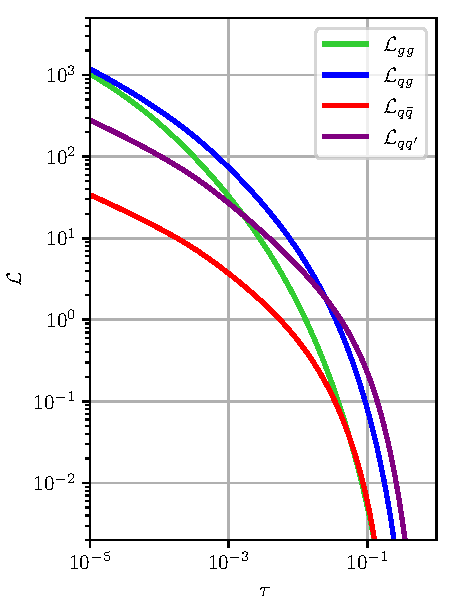
\includegraphics[width=\textwidth]{Images/luminosity.pdf}
\captionof{figure}{Displayed is the partonic luminosity for combinations of various partons. The luminosities are defined as $\mathcal{L}_{qg} = 2 \times \sum_i (\mathcal{L}_{q_i g} + \mathcal{L}_{\bar{q}_i g})$, $\mathcal{L}_{q \bar{q}} = 2 \times \sum_i \mathcal{L}_{q_i \bar{q}_i}$, $\mathcal{L}_{q q^\prime} = \sum_{i, j} (\mathcal{L}_{q_i q_j} + \mathcal{L}_{q_i \bar{q}_j} + \mathcal{L}_{\bar{q}_i \bar{q}_j}) - \mathcal{L}_{q \bar{q}}$. The setup is the same as in Fig.~\ref{fig:2:PDF}.}
\label{fig:2:luminosity}
\end{minipage}
\end{figure}

The factorization theorem~\eqref{eq:2:factorization} is central in the \acs{SM} as it tells us that the \acs{PDF}s are universal quantities, \ie\ they are not specific to any one process. It is a postulate of the parton model, in which hadrons are thought of as collection of the free elementary particles. In \acs{QCD} however, the theorem requires proof~\cite{Collins:1989gx}!
The \acs{PDF} for all light partons are displayed in Fig.~\ref{fig:2:PDF}. In Fig.~\ref{fig:2:luminosity} we show the partonic luminosity for exemplary parton combinations. \acs{PDF}s describe long range interactions, a regime in which \acs{QCD} is non-perturbative. As such, \acs{PDF}s are non-perturbative objects which have to be measured in experiments or be calculated non-pertubatively, \eg\ on the lattice.

The factorization scale in unphysical in the sense that it is not a parameter in our theory, nor can it be measured in an experiment. As usual we can apply the \acs{RGE} to determine the running of the renormalized \acs{PDF}s
\begin{equation}
0 = \frac{\dd}{\dd \ln \mu_F} f_{H,i}(x) = \frac{\dd}{\dd \ln \mu_F} (Z_{ij} \otimes f_{H, j}(\cdot, \mu_F))(x).
\end{equation}
This can be rewritten to
\begin{equation}
\begin{split}
\frac{\dd f_{H,i}(x, \mu_F)}{\dd \ln \mu_F} &=  2 \alphas \left(Z_{ij}^{-1} \otimes \frac{\dd Z_{jk}^{(1)}}{\dd \alphas} \otimes f_{H,k}(\cdot, \mu_F) \right)(x, \mu_F) \\
&= \frac{\alphas}{\pi} \left(P_{ij}^{(0)} \otimes f_{H,j}(\cdot, \mu_F) \right)(x) + \BigO{\alphas^2},
\label{eq:2:DGLAP}
\end{split}
\end{equation}
where $Z^{(1)}_{ij}$ is the residue of the renormalization constant. So even though the \acs{PDF}s are non-perturbative, their dependence on the factorization scale is. Eq.~\eqref{eq:2:DGLAP} is the famous \textit{Dokshitzter-Gribow-Lipatow-Altarelli-Parisi-evolution equation} (DGLAP equations)~\cite{Dokshitzer:1977sg,Gribov:1972ri,Altarelli:1977zs}.

In the derivation above, we have treated the partons inside the hadrons as massless, which leads to real collinear singularities. In reality, all quarks have finite masses, so the phase-space integration only yields logarithmic mass enhancements of the form $\ln (\hat{s}/m_q^2)$ instead of actual singularities. The DGLAP equations then automatically resum these logarithms. For most applications at the \acs{LHC}, the typical hard scattering scale is orders of magnitudes larger than all quark masses except for the top quark mass. It is therefore beneficial to treat them as massless partons, as the appearance of the large logarithms would otherwise completely destroy the perturbative convergence. However, treating quarks as massless also implies that we neglect their mass-dependent effects in the hard-scattering matrix elements. If the scattering process is sensitive to the quark masses---for example, in processes involving Higgs couplings to quarks---these mass effects might be lost.

The number of quark flavors treated as active (massless) partons defines our \textit{flavor scheme} (\acs{FS}). For instance, if we treat the lightest four flavors (up, down, strange, charm) as massless, while considering the bottom and top quarks as massive, we are working in the 4\acs{FS}. Analogously, if the bottom quark is also considered massless, we are working in the 5\acs{FS}, and so on.

\subsection{The Phase-Space Integration}\label{subsec:2:phase_space_integration}
Even after renormalization and collinear renormalization can the amplitude exhibit divergences. The scatting amplitude in and of itself is not a physical observable; therefore, it is not required to be finite. Physical observables are cross sections, which are obtained by performing phase-space integrations over the squared amplitudes. However, even after integrating over the phase space, the cross section is not guaranteed to be finite. The reason is that the Born process is indistinguishable from processes with additional infrared radiation. Indeed, no matter how precise a detector is, below a certain resolution, it becomes impossible to detect a very soft photon or to distinguish two highly collinear jets. Hence, computing a cross section with a fixed final state does not make physical sense. Instead, one must consider sufficiently inclusive observables---so called \textit{IR-safe observables}. For these, Kinoshita, Lee and Nauenberg proved that in unitary theories all IR singularities cancel~\cite{Kinoshita:1975bt, Lee:1964is}. This is known as the Kinoshita-Lee-Nauenberg (KLN) theorem.

An example of an observable which is trivially IR safe is the fully inclusive cross section
\begin{equation}
\hat{\sigma}_{ij \rightarrow n+X} = \sum_{k = 1}^\infty \hat{\sigma}_{ij \rightarrow n + k}, \quad \text{for} \quad \hat{\sigma}_{ij \rightarrow n}^{(0)} \quad \text{finite},
\end{equation}
where $n + k$ indicates that in addition to the final state $n$ we now have $k$ massless partons of whatever flavor. In perturbation theory, the infinite sum is truncated at a given order and at each order
\begin{equation}
\hat{\sigma}_{ij \rightarrow n+X}^{(l)} = \sum_{k = 0}^l \hat{\sigma}_{ij \rightarrow n + k}^{(l - k)},
\end{equation}
summed together with the contribution from collinear renormalization will be finite. For example at \acs{NLO}, the finite inclusive cross section reads
\begin{equation}
\hat{\sigma}_{ij \rightarrow n+X}^{(1)} = \hat{\sigma}_{ij \rightarrow n}^{R} + \hat{\sigma}_{ij \rightarrow n}^{V} + \hat{\sigma}_{ij \rightarrow n}^C,
\end{equation}
where
\begin{equation}
\hat{\sigma}_{ij \rightarrow n}^R = \frac{1}{F}\int \dd \Phi_{n + 1} \, \sum_c |M_{ij \rightarrow n + c}^{(0)}|^2
\end{equation}
is the real correction,
\begin{equation}
\hat{\sigma}_{ij \rightarrow n}^V = \frac{1}{F} \int \dd \Phi_n \, 2 \Re \left( \left(M_{ij \rightarrow n}^{(0)}\right)^* M_{ij \rightarrow n}^{(1)} \right)
\end{equation}
is the virtual correction, and
\begin{equation}
\hat{\sigma}_{ij \rightarrow n}^C = \frac{1}{F} \int \dd \Phi_n \, \frac{\alphas}{2 \pi} \frac{1}{\epsilon} \left(\frac{\mu_R^2}{\mu_F^2} \right)^\epsilon \sum_c \int_0^1 \dd z\,  \left[ P_{ci}^{(0)}(z) |M_{cj \rightarrow n}^{(0)}|^2 + P_{cj}^{(0)}(z) |M_{ic \rightarrow n}^{(0)}|^2 \right]
\end{equation}
are the corrections from collinear renormalization. Figure~\ref{fig:2:loops_and_legs} provides a pictorial representation of the required partonic cross sections for Higgs boson production in the gluon fusion channel at various perturbative orders.
\begin{figure}[h]
\centering
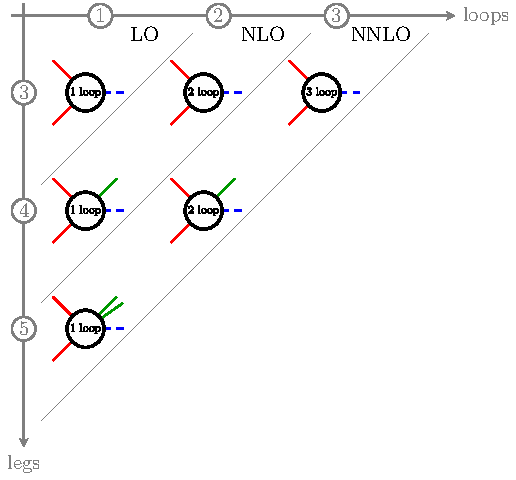
\includegraphics[width=12cm]{Images/loops_and_legs.pdf}
\caption{Pictorial representation of the needed partonic cross sections at various perturbative orders of the fully inclusive hadronic cross section. The graphic shows the example of Higgs production in the gluon fusion channel.}
\label{fig:2:loops_and_legs}
\end{figure}

Although the sum of the contributions to the cross section is guaranteed to be finite due to the KLN theorem, the presence of IR singularities in individual terms poses significant challenges for practical calculations. These singularities prevent a straightforward evaluation of the phase-space integrals. To overcome this, we once again have to introduce regulators (such as dimensional regularization) to make the integrals well-defined. Over the years, numerous techniques have been developed to compute phase-space integrals efficiently. These techniques can generally be categorized into two main types: \textit{Analytic methods}, and \textit{numerical methods}.

As the name suggests, in the former class, the phase-space integrals are solved analytically. One noteworthy member of this class is the \textit{reverse-unitarity method}~\cite{Anastasiou:2002yz}, which was first applied to Higgs production in the gluon fusion channel. The method uses unitarity, to rewrite the phase-space integrals in terms of loop integrals over cut-propagators. One can then apply the remarkable techniques developed for Feynman integrals to these phase-space integrals and solve them analytically. The mayor downside of this approach is that it is highly process and observable dependent, meaning that for every process and every observable we have to start over from scratch. Furthermore, by the very nature of the method, you are always restricted to inclusive jet observables. Nevertheless, it has been successfully applied to, among others, Higgs-rapidity and Higgs-$p_T$ distributions~\cite{Dulat:2017brz}.

Among the numerical methods, there are two mayor approaches: \textit{slicing} and \textit{subtraction methods}. The former rely on a variable that isolates the \acs{IR}-sensitive region of the phase space. Consider once again the example of Higgs production. Here, the IR-sensitive region of the phase space corresponds to configurations where the transverse momentum of the Higgs boson, $p_T$, approaches zero. The phase-space integral can then be decomposed into
\begin{equation}
\int_0^{p_T} \dd k_T \, \dd \hat{\sigma}_{ij \rightarrow H + c} = \int_0^{p_T^\text{cut}} \dd k_T \, \dd \hat{\sigma}_{ij \rightarrow H + c} + \int_{p_T^\text{cut}}^{p_T} \dd k_T \, \dd \hat{\sigma}_{ij \rightarrow H + c}.
\end{equation}
The first integral on the right-hand side is now finite and can be computed numerically, \eg\ using \textit{Monte-Carlo} (\acs{MC}) techniques. If we choose $p_T^{\text{Cut}}$ small enough, then we can approximate the integrand in the second integral, by its \acs{IR} limit and solve the integral analytically. The pole of the integral should then cancel against the poles in the virtual integration and the counter term from collinear renormalization. The mayor advantage of this method is its simplicity. One big  downside is its dependence on the unphysical cutoff scale. Ideally it is chosen very small, such that the approximation introduces little to no error. But if chosen too small, the integrations will have huge logarithmic enhancements which can easily spoil the numerical precision. Another disadvantage is that not all processes or observables have easily identifiable slicing variables, or the analytic integration is very challenging. For example, $p_T$ slicing only works for color singlet production, indeed if we have a jet in the final state, we can encounter collinear divergences also at finite transverse momenta of the jet. For processes involving jets, a possible slicing variable is the $N$-jettiness
\begin{equation}
\mathcal{T}_N \equiv \sum_k \min_i\! \bigg \lbrace \frac{2 p_i \cdot q_k}{Q_i} \bigg \rbrace,
\end{equation}
with $N$, the number of jets, $q_k$, the momenta of the unresolved partons, $p_i$, the momenta of the resolved jets, and $Q_i$ a normalization factor which can for example be set to the jet energy. However, the analytic integration becomes highly non-trivial and is a matter of active research. Currently, the $N$-jettiness beam functions are known at N${}^3$LO~\cite{Ebert:2020unb}, the $0$-jettiness soft function is known at N${}^3$LO~\cite{Baranowski:2024vxg, Baranowski:2024ysi} and \acs{NNLO} $1$-jettiness soft functions and jet functions are also known~\cite{Campbell:2017hsw, Becher:2010pd, Becher:2006qw, Boughezal:2015eha}.

Subtraction methods on the other hand, work by subtracting the infrared limits at the integrand level. In the \textit{Frixione-Kunszt-Signer subtraction scheme} (FKS subtraction scheme) one first isolates the \acs{IR} divergence by partitioning the phase space into \textit{sectors} using \textit{selector functions}. These functions isolate specific infrared limits by approaching unity when a particular limit is approached (\eg, when an unresolved parton becomes soft or collinear) and vanish in other limits. For a single unresolved parton, a possible selector function is
\begin{equation}
\mathcal{S}_{n+1,k} \equiv \frac{1}{d_{n+1,k}} \left(\sum_{k} \frac{1}{d_{n+1,k}} \right)^{-1}, \quad \text{where} \quad d_{n+1,k} \equiv \left(\frac{E_{n+1}}{\sqrt{\hat{s}}}\right)^\alpha (1 - \cos \theta_{n+1,k})^\beta.
\end{equation}
The first index $n+1$ is the index of the unresolved parton, while the second index is the index of the reference parton. $E_{n+1}$ denotes the energy of the unresolved parton, this factor is therefore to identify soft singularities. Consequently, the power $\alpha$ can be set to zero if the unresolved parton is a quark. Other than that, the powers must be strictly positive $\alpha, \beta > 0$. If $n+1$ now becomes collinear to one of the partons, say parton $i$, then the selector function $S_{n+1,i}$ will approach one. And since the selector functions are strictly positive and form a decomposition of unity
\begin{equation}
\sum_k \mathcal{S}_{n+1,k} = 1,
\end{equation}
all other selector functions will go to zero simultaneously.

The real emission cross section can then be written as a sum over sectors:
\begin{equation}
\hat{\sigma}_{ij \rightarrow n+u} = \frac{1}{F} \sum_k \int \dd \Phi_{n + 1} \, |M_{ij \rightarrow n + u}^{(0)}|^2 \mathcal{S}_{n+1, k}.
\end{equation}
Now say we found a way to factorize the phase space, such that the infrared limits of a specific sector, are isolated (see for example Ref.~\cite{Czakon:2019tmo}). Then in each sector, we will have two unit integrations over $\xi$ and $\eta$ which parameterize the soft and collinear limit respectively, \ie\ if $\xi\rightarrow 0$, then the momentum of the unresolved parton goes to zero and if $\eta \rightarrow 0$, the unresolved parton will become collinear to the reference momentum of that sector. The amplitude has the singular scaling $|M_{ij \rightarrow n + u}^{(0)}|^2 \sim \xi^{-2} \eta^{-1}$, leading to an integral of the form
\begin{equation}
\int_0^1 \frac{\dd \eta}{\eta^{1 + \epsilon}} \frac{\dd \xi}{\xi^{1 + 2 \epsilon}} f(\eta, \xi, \cdots),
\end{equation}
where $f$ is a function regular in the limits $\eta, \xi \rightarrow 0$. If we now apply the distributional identity
\begin{equation}
\frac{1}{x^{1 - \epsilon}} = \frac{1}{\epsilon} \delta (x) + \sum_{k = 0} \frac{\epsilon^k}{k!} \left( \frac{\ln^k x}{x} \right)_+,
\label{eq:2:distributional_identity}
\end{equation}
we can explicitly carry out all integrations.

The \textit{sector improved residue subtraction scheme}~\cite{Czakon:2010td} extends the FKS subtraction scheme to \acs{NNLO}. As of today, it is the only subtraction scheme capable of computing any QCD phase-space integral. Beyond \acs{NNLO}, developing efficient and general subtraction schemes remains an open challenge in perturbative QCD.








